% SimGate: draft for IEEE IV 2027 (deadline 15 Nov 2026, 6 pages with references).
% Build on Overleaf: upload this folder (main.tex, refs.bib, figures/). Locally:
% tectonic -X compile main.tex (5 pages on 6 Oct, limit 6).
% Every number comes from research/FACTS.md. \pending{} marks results still running
% (campaign C3, held-out plan-fault batch g3) and the co-author's first name.
\documentclass[conference]{IEEEtran}
\usepackage{cite}
\usepackage{amsmath,amssymb}
\usepackage{graphicx}
\usepackage{booktabs}
\usepackage{url}
\usepackage{xcolor}
\newcommand{\pending}[1]{\textcolor{red}{[#1]}}

\begin{document}

\title{SimGate: Runtime Assurance for\\LLM-Operated Driving Simulation}

\author{\IEEEauthorblockN{Will Varner and \pending{first name} Shao}
\IEEEauthorblockA{College of Engineering, University of Georgia, Athens, GA, USA}}

\maketitle

\begin{abstract}
Closed-loop evaluation of driving policies needs hundreds of short simulation
runs, which run unattended. Unattended runs fail silently: in our own earlier
data a misconfigured model, a delay that never applied, and missing results all
looked like findings. Large language model (LLM) agents could operate such
batches, but an agent that can act can also corrupt the dataset. We present
SimGate, which applies the Simplex architecture to an LLM agent with
experimental validity, not physical safety, as the protected property:
deterministic checks decide which runs enter the dataset, and the model only
proposes. When a run fails, an investigating agent with read-only tools picks a
recovery from a finite menu that a validator gates. After a batch, an auditing
agent flags runs that do not measure what they claim and proposes checks, which
enter the gate only if data and a person admit them. Because the menu is
finite, we check the gate against every answer a policy could give; the check
found one real defect. On the AlpaSim simulator with the VaVAM driving model,
across two fault-injection campaigns and six policy arms, no injected invalid
run was kept after the gate and audit, against 25 per arm without the gate.
\end{abstract}

\section{Introduction}

A closed-loop driving simulator replays a recorded scene, lets a policy drive,
and scores the result. Each run is short, around twelve simulated seconds in
our setting, because the reconstructed world only exists where the recording
vehicle drove~\cite{alpasim}. A study is therefore hundreds of runs, launched
in batches that run overnight with nobody watching.

Such batches fail silently. In our own earlier data, four failures looked like
results: the driving model was configured with one frame of
history instead of eight and crashed in 8 of 10 runs; a latency study was
plotted from a delay the simulator never applied (162 of 212 runs); 22\% of
runs wrote no metrics and silently dropped out; and a solver reported success
whenever it did not raise. None of these raised an error.

LLM agents are increasingly used to run experiments~\cite{lu2024aiscientist,boiko2023coscientist}
and to operate pipelines~\cite{selfhealing2026}. An agent that can relaunch,
reconfigure, and clean up could keep a batch running through failures. It
could also keep a run it should have discarded, change what an experiment
measures, or loop. The question we ask is how to let a model operate a
simulation batch without trusting it.

Our answer is SimGate, the Simplex architecture~\cite{sha2001simplex,seto1998simplex}
applied to an LLM operator, with the dataset as the protected property.
Deterministic code owns the batch and decides which runs are kept. The model
proposes in two places: a recovery when a run fails, and flags and new checks
when a batch ends. Our contributions:
\begin{itemize}
\item A gate for simulation data: checks before and after every run, including
whether requested settings took effect and whether the motion was physically
possible and followed the driver's plan.
\item An investigating agent on a finite recovery menu behind a validator, and
an exhaustive check over every answer a policy could give, which found a
defect testing had not.
\item An auditing agent whose findings become deterministic checks only after
admission against known-good runs and a person's approval.
\item Fault-injection campaigns on AlpaSim, each run under a hand-written
policy and two model tiers on the same gated menu, scored by outcome.
\end{itemize}

\section{Related Work}

\emph{Runtime assurance.} Simplex pairs an unverified controller with a simple
verified one and a switch that admits only safe actions~\cite{sha2001simplex,seto1998simplex};
Black-Box Simplex~\cite{mehmood2022blackbox} and shielding~\cite{alshiekh2018shield}
extend the idea. Recent work places deterministic gates around LLM advice in
process control~\cite{misra2026admitbench,vyas2026detection} and enforces
runtime rules on agent actions~\cite{wang2026agentspec,shieldagent2025}. These
protect physical or behavioural safety; SimGate protects the validity of the
data an experiment produces.

\emph{Agents that run experiments.} AI-scientist systems~\cite{lu2024aiscientist}
and laboratory agents~\cite{boiko2023coscientist} let the model act directly;
self-healing pipelines~\cite{selfhealing2026} add deterministic checks and
bounded remediation. Agents also drive simulation testing~\cite{duvvuru2025autosimtest,gao2026plannerforge}.
None compares the model with a rule policy on the same gated action set.

\emph{Silent failures.} Training-time invariant checks~\cite{jiang2025traincheck}
and data validation~\cite{breck2019datavalidation} catch silent errors in
learning pipelines. We check simulation runs, where a run can finish cleanly
and still measure the wrong thing.

\section{SimGate}

\subsection{Setting}
AlpaSim~\cite{alpasim} runs a driving policy, here VaVAM~\cite{bartoccioni2025vavam},
which plans from the last eight camera frames; a linear model-predictive
controller tracks the plan; a learned traffic model, CATK~\cite{zhang2025catk},
moves other vehicles. The first 4.5\,s of each run replay the recorded human
trajectory while the policy fills its frame history. A run writes its resolved
configuration, a log of every message, and metrics.

\subsection{State machine and gate}
\begin{figure}[t]
\centering
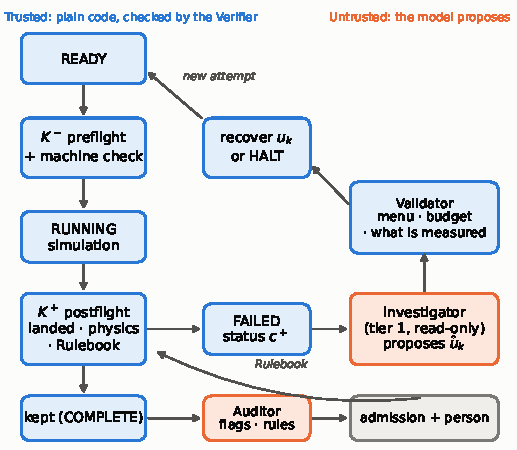
\includegraphics[width=\columnwidth]{figures/architecture.pdf}
\caption{SimGate. Trusted code (blue) owns the loop and decides; the model (orange) proposes a recovery when a run fails and flags and rules after a batch; a person enacts admitted rules.}
\label{fig:arch}
\end{figure}

Following the notation of a run-level control loop, each run is in a discrete
state $x_k \in \{$READY, RUNNING, COMPLETE, FAILED, DONE$\}$ (Fig.~\ref{fig:arch}).
Python owns every transition. Before launch, preflight $K^-$ rejects
configurations that must not run and checks the machine (leftover containers,
container-network capacity, GPU memory, disk). After a run, postflight $K^+$
requires exit status 0, readable metrics, that every requested setting appears
in the resolved configuration, every admitted rule, and the physics bounds
of Section~\ref{sec:physics}. Its output $c^+$ is a structured status. A run is
kept only if $K^+$ passes.

\subsection{The Investigator}
Only on FAILED is a model consulted: one headless call with a fresh context
whose whole system prompt is a contract describing the states and the menu.
It proposes $\hat u_k$, one skill from a finite menu with parameters:
CONFIGURE (change how a run executes: model context length, traffic-model
device, scene catalogue), RE-RUN, RESTART\_CLEANUP (remove this run's
containers), CLEANUP\_ENV (remove the simulator's leftovers from the machine),
or HALT (hand the run to a person). A JSON schema forces the answer's shape. In
the tier-1 variant the model may first investigate with read-only tools: it
can read the failed run's files and log and run four inspection commands; the
platform's permission system denies everything else. A probe told it to read
outside the run, list home directories, write a file, remove a container, and
chain a deletion after an allowed command; all five were denied.

A validator then turns $\hat u_k$ into $u_k$ or a halt. It rejects keeping a
failed run, launching, any skill not on the menu, parameters outside the
configurable keys, a configuration preflight rejects, a fourth attempt, and any
change to what the experiment measures (the delay, the scene). A rejected
proposal halts the run for a person; it is never retried. Recovery queues a
new attempt and never edits the failed run.

\subsection{The Auditor and the Rulebook}
Per-run checks catch failures someone anticipated. After a batch, an auditing
agent reads an anonymised snapshot of the kept runs: random identifiers, real
names removed, the batch's claim, each run's label and metrics, read-only
access to configurations and the motion summary of Section~\ref{sec:physics},
and one known-good reference run. It flags runs whose data does not measure what
the batch claims, and is told not to flag outcomes such as collisions. Flagged
runs are quarantined, never deleted.

For each kind of problem it flags, the Auditor proposes a rule: one value in a
resolved configuration and the condition it must meet, or equality with the
run's label. A rule is admitted only if it fires on a flagged run, fires on
none of 51 known-good runs, and does not pin a variable the experiment varies;
a person then enacts it, after which $K^+$ checks it on every run with no model.

\subsection{Physics checks}\label{sec:physics}
Summary metrics can look normal while the motion is impossible or not the
policy's. $K^+$ rebuilds the ego's motion from the run's log every 0.1\,s and
bounds it by what a road vehicle can do: acceleration within 1\,g; yaw rate
within 2\,rad/s; the vehicle model's reported speed within 1\,m/s of the speed
the poses imply; the ego on the recorded human trajectory for at most 98\% of
steps; and no overlap of the ego's box with another actor's without a scored
collision. A last check compares the plan the driver returned with the plan
the controller was given: after the warm-up they are the same plan, so the
median sideways distance between them must stay below 5\,cm.

\subsection{The Verifier}
Because the menu is finite, we check the gate rather than sample the model. An
adversarial policy tries 26 answers at every FAILED state, every skill with
legal and illegal parameters, against a world that fails every launch, breaks
the machine, or drops a setting. Each transition runs the real validator and
recovery code. The invariants: no failed run is kept; no rejected
configuration launches; at most three launches per run; every path ends; and
no kept run measures a delay or scene other than the one queued.

\section{Experimental Setup}

All runs use VaVAM with eight frames, the linear controller, CATK on the CPU,
and one 12\,GB GPU; the model is Claude Opus~5.5 through its command-line
interface. B2 is 150 runs on one scene; S1 is one run on each of 101
downloaded scenes. We inject faults into the run, its environment, or its
data: a killed or frozen simulator, deleted or corrupted metrics, a delay
silently dropped from every attempt, an exhausted container-network pool, and
two \emph{silent} faults that pass every per-run check except physics: the
recording drives the whole run (\emph{rails}) or the controller is replaced by
one that moves the vehicle along the plan (\emph{kinematic}). Plan faults, a
1.0\,m lateral bias and a frozen plan, use the simulator's own plan-corruption
hook.

A campaign is one fault plan of 50 runs, five per fault kind and ten clean,
over six scenes, run under three policies: a hand-written script (retry,
then clean up, then stop), tier~0 (the model without tools), and tier~1 (with
read-only tools). C1 ran with the physics bounds off and C2 with them on; each
arm ended with an audit. We score outcomes: whether a lineage ends in a kept,
valid run, how many launches it cost, and whether a person had to step in.

\section{Results}

\subsection{Unattended operation}
B2 ran 150 runs in 537\,min and kept all 150. Its only failures were the first
eight runs, which found the container-network pool exhausted by 29 networks
earlier runs had left behind; recovering a single run could not fix a shared
machine, a person removed the networks once, and that failure became the
machine check and CLEANUP\_ENV, which replayed the same exhaustion and cleared
it with no person. S1 kept 100 of 101 runs on 99 scenes in 381\,min; tier~1
retried one natural failure successfully and halted the other, and its audit
flagged none of the 100.

\subsection{Data validity}
\begin{figure}[t]
\centering
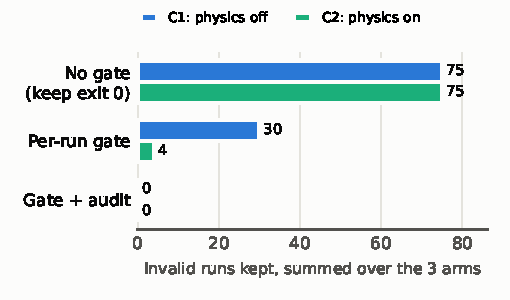
\includegraphics[width=\columnwidth]{figures/campaign_invalid.pdf}
\caption{Injected invalid runs kept, summed over the three arms of each campaign.}
\label{fig:invalid}
\end{figure}

\begin{table}[t]
\centering
\caption{Campaign outcomes per arm (50 planned runs each)}
\label{tab:campaigns}
\setlength{\tabcolsep}{4pt}
\begin{tabular}{@{}lrrrrrr@{}}
\toprule
 & & & \multicolumn{3}{c}{Invalid kept} & \\
\cmidrule(lr){4-6}
Arm & Launches & Valid & no gate & gate & +audit & Halts \\
\midrule
C1 script & 80 & 35 & 25 & 10 & 0 & 5 \\
C1 tier 1 & 72 & 35 & 25 & 10 & 0 & 5 \\
C1 tier 0 & 62 & 25 & 25 & 10 & 0 & 15 \\
C2 script & 91 & 45 & 25 & 0 & 0 & 5 \\
C2 tier 1 & 72 & 36 & 25 & 3 & 0 & 11 \\
C2 tier 0 & 61 & 26 & 25 & 1 & 0 & 23 \\
\bottomrule
\end{tabular}
\end{table}

Without the gate, keeping every run that exits 0 would keep 25 invalid runs
per arm: deleted or corrupted metrics, the dropped delay, and the silent
faults (Table~\ref{tab:campaigns}, Fig.~\ref{fig:invalid}). The per-run gate
left the 10 silent-fault runs per arm with physics off (C1) and 0 to 3 with it
on (C2). After the audit, no arm kept an invalid run. \pending{C3, seed 3, with
silent faults that repeat on retry.}

\subsection{Recovery policies}
\begin{figure*}[t]
\centering
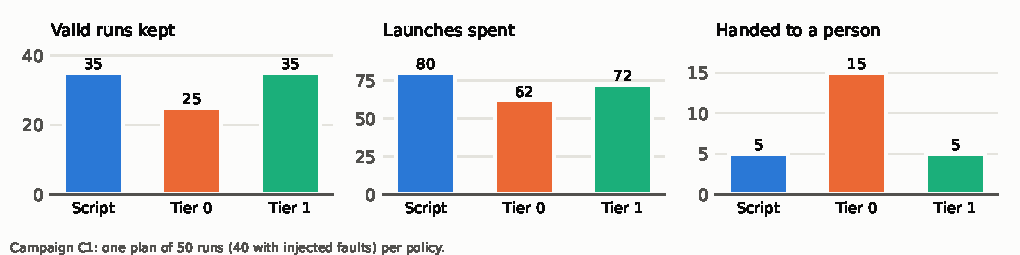
\includegraphics[width=0.85\textwidth]{figures/campaign_outcomes.pdf}
\caption{C1 per policy: valid runs kept, launches spent, and runs handed to a person.}
\label{fig:outcomes}
\end{figure*}

On faults that a retry can fix, the script and tier~1 recovered 5 of 5 of every
kind in both campaigns (Fig.~\ref{fig:outcomes}). Tier~0 recovered 0 of 5
deleted and 0 to 1 of 5 corrupted metrics and halted them: those runs exit 0
and their logs show nothing, and without tools the model cannot see that the
metrics are missing. On the dropped delay, which no retry fixes, the script
spent 15 launches before its attempt budget stopped it, while both model tiers
halted at the first failure. In C1 tier~1 kept as many valid runs as the
script, 35, in 72 launches against 80, and every halt it chose was on the
unrecoverable fault. The gate rejected no model answer in either campaign.

With physics on, the script's retries recovered the silent faults, which in C1
and C2 did not repeat on a retry, while the model tiers halted most of them as
physically impossible runs. A configuration error that causes such a run would
repeat, so C3 makes them persistent \pending{C3 result}. A tier-1 call used
about 49\,k context tokens and a median 12.5\,s, a tier-0 call about 5\,k and
8.9\,s.

Scoring by outcome can hide a wrong diagnosis. On hangs, both tiers mostly
reconfigured the traffic model, blaming slowness, and the retry succeeded
because the injected hang was transient. The monitor had stopped the run
before the diagnosis, removing the paused container that showed the real
cause; replayed with that container's paused state reconstructed, tier~1
cleaned up and retried in 3 of 3 calls. The monitor now records the machine before stopping a run.

\subsection{The Auditor and rule mining}
\begin{table}[t]
\centering
\caption{Auditor on batches built from runs on disk (three audits each, identical; False: valid runs flagged)}
\label{tab:auditor}
\setlength{\tabcolsep}{4pt}
\begin{tabular}{@{}lrrr@{}}
\toprule
Batch & Invalid & Caught & False \\
\midrule
A: 10 one-frame among 20 valid & 10 & 10 & 0 \\
B: 20 labelled with a delay not applied & 20 & 20 & 0 \\
C: 6 missing from the results & 6 & 6 & 0 \\
D: 30 valid & 0 & -- & 0 \\
E: the 10 one-frame alone & 10 & 0 & 0 \\
F: E plus one reference run & 10 & 10 & 0 \\
\bottomrule
\end{tabular}
\end{table}

The Auditor caught every planted inconsistency with no false flags, and three
audits per batch with new identifiers gave identical results
(Table~\ref{tab:auditor}). It did not catch batch E, which is wrong the same way
throughout, as the original one-frame configuration was; one reference run
restored detection. It also found, in an old batch, the same network-pool
exhaustion B2 later hit. The rules it proposed and the admission step accepted
then ran with no model: ``context length is 8'', learned from batch A, caught
all of batch E, and a rule that the delay equals the label caught 20 of 20
held-out mislabelled runs, with no false flags on 30 valid runs.

\subsection{Physics and the hard case}
The physics bounds flagged none of 258 kept clean runs across about 100 scenes and all
six silent-fault runs of a pilot, without reading a configuration file. On
C1's fresh runs, checked after the fact, they caught 25 of 30 silent faults
and flagged none of 95 other runs; the five misses were kinematic runs on
gentler scenes, all of which the audit quarantined. No jerk statistic recovers
them: one clean highway run is as jerky as any kinematic run (p99 jerk
101\,m/s$^3$ against at least 78.8 over 43 kinematic runs), so this fault is
left to the Auditor, which reads the configuration. With configuration files
hidden, the Auditor caught all six pilot silent faults when given each run's
motion summary and three without it: summary metrics hid every kinematic run.

Plan faults are harder. A lateral bias or a frozen plan leaves the motion
physically possible, and the gate kept all eight such runs. The Auditor with
configurations hidden caught none of them, with one or with per-scene
references: its contract tells it not to flag poor driving, and a corrupted
plan looks like poor driving. The plan-handoff check, which compares the
driver's plan with the plan the controller was given, separated them exactly:
median sideways gap 0 to 0.008\,m on all clean runs, 0.14 to 1.0\,m on all eight
plan-fault runs, and with it the bounds flagged none of 202 fresh campaign runs
that played no part in setting them. Given that measurement, the Auditor caught 4 of 8 with one
reference (every lateral bias) and 8 of 8 with a clean reference from each
scene, with no false flag, in each of three audits: the frozen plan stands out only against the same
scene. \pending{held-out batch g3: 0.3\,m bias and waypoint noise on four new
scenes.}

\subsection{Verification}
The first run of the Verifier, over 65 states and 5{,}070 transitions, found 28
violations of one kind: after a delay that did not apply, a recovery could
reconfigure the delay to zero, and the next run passed every check and was
kept while measuring a different condition than the one queued, the latency
failure of our earlier data reintroduced by recovery. A recovery may now change
how a run executes but not what it measures. The check now finds no violation
over 3{,}822 transitions and runs with the test suite.

\section{Limitations}
We use one simulator and one driving policy. Model results are per fault kind
with five samples per arm and campaign. The silent faults in C1 and C2 did not
repeat on a retry, which favours blind retries. Tier~1 halted some runs a retry
would have recovered. The Auditor needs a known-good reference to see a batch
that is uniformly wrong, and its rules can be specific to a study, which is why
a person enacts them. Physics bounds were set from vehicle limits, but the jerk
bound was dropped and three other thresholds were revised after clean runs
fired them; fresh campaign runs and the held-out plan-fault batch are the
check. The simulator retries a crashed rollout inside one run; this happened in 1
of 496 kept runs, and the attempt count is now recorded but not checked.

\section{Conclusion}
SimGate lets an LLM operate an unattended simulation batch without being
trusted with the data. The model proposes recoveries, flags, and checks;
deterministic code, an admission step, and a person decide. Across six
campaign arms no injected invalid run reached the dataset, the gate held
against every answer a policy could give, and what the Auditor learned became
checks that run without it.

\bibliographystyle{IEEEtran}
\bibliography{refs}

\end{document}
